%%%%%%%%%%%%%%%%%%%%%%%%%%%%%%%%%%%%%%%%%%%%%%%%%%%%%%%%%%%%%%%%
%%                                                            %%
%%   essentialsOfLatin, Italian translation 2017              %%
%%                                                            %%
%% From:  Henry C. Pearson, Essentials Of Latin For Beginners %%
%%        (1915, New York, American Book Company)             %%
%%                                                            %%
%%    https://archive.org/details/essentialslatin04peargoog   %%
%%                                                            %%
%% Translated by g.p.ciceri <gp.ciceri@gmail.com>             %%
%% ---------------------------------------------------------- %%
%% This translation is Licensed under                         %%
%% Creative Commons Attribution-ShareAlike 4.0 International  %%
%% https://creativecommons.org/licenses/by-sa/4.0/            %%
%%                                                            %%
%%%%%%%%%%%%%%%%%%%%%%%%%%%%%%%%%%%%%%%%%%%%%%%%%%%%%%%%%%%%%%%%

% āēīōū
% ăĕĭŏŭ




\documentclass[nols]{tufte-handout}

%\geometry{showframe} % display margins for debugging page layout

\usepackage{fontspec}
\usepackage{ifxetex}
\setmainfont[Path=./fonts/palatino-linotype/, ItalicFont=palai.ttf, BoldFont=palab.ttf]{pala.ttf}


% \defaultfontfeatures{Mapping=tex-text}
% \setromanfont[Path=./fonts/TeX-Gyre-Schola/,Mapping=tex-text]{TeX Gyre Schola}
% \setsansfont[Path=./fonts/TeX-Gyre-Heros/,Scale=MatchLowercase,Mapping=tex-text]{TeX Gyre Heros}
% \setmonofont[Path=./fonts/TeX-Gyre-Cursor/,Scale=MatchLowercase]{TeX Gyre Cursor}

\usepackage{lipsum}
\usepackage{url}
\usepackage{longtable}
\usepackage{stackengine}

\usepackage{graphicx} % allow embedded images
  \setkeys{Gin}{width=\linewidth,totalheight=\textheight,keepaspectratio}
  \graphicspath{{graphics/}} % set of paths to search for images
\usepackage{amsmath}  % extended mathematics
\usepackage{booktabs} % book-quality tables
\usepackage{units}    % non-stacked fractions and better unit spacing
\usepackage{multicol} % multiple column layout facilities
\usepackage{lipsum}   % filler text
\usepackage{fancyvrb} % extended verbatim environments
  \fvset{fontsize=\normalsize}% default font size for fancy-verbatim environments

% Standardize command font styles and environments
\newcommand{\doccmd}[1]{\texttt{\textbackslash#1}}% command name -- adds backslash automatically
\newcommand{\docopt}[1]{\ensuremath{\langle}\textrm{\textit{#1}}\ensuremath{\rangle}}% optional command argument
\newcommand{\docarg}[1]{\textrm{\textit{#1}}}% (required) command argument
\newcommand{\docenv}[1]{\textsf{#1}}% environment name
\newcommand{\docpkg}[1]{\texttt{#1}}% package name
\newcommand{\doccls}[1]{\texttt{#1}}% document class name
\newcommand{\docclsopt}[1]{\texttt{#1}}% document class option name
\newenvironment{docspec}{\begin{quote}\noindent}{\end{quote}}% command specification environment

% concetti morfosintattici
\usepackage{xspace} 
\newcommand{\noun}{\textsc{sostantivo}\xspace}
\newcommand{\nouns}{\textsc{sostantivi}\xspace}
\newcommand{\adject}{\textsc{aggettivo}\xspace}
\newcommand{\adjects}{\textsc{aggettivi}\xspace}
\newcommand{\gnumber}{\textsc{numero}\xspace}
\newcommand{\gnumbers}{\textsc{numeri}\xspace}
\newcommand{\gender}{\textsc{genere}\xspace}
\newcommand{\genders}{\textsc{generi}\xspace}
\newcommand{\gcase}{\textsc{caso}\xspace}
\newcommand{\gcases}{\textsc{casi}\xspace}
\newcommand{\tense}{\textsc{tempo}\xspace}
\newcommand{\mood}{\textsc{modo}\xspace}
\newcommand{\gverb}{\textsc{verbo}\xspace}
\newcommand{\gverbs}{\textsc{verbi}\xspace}
\newcommand{\adjective}{\textsc{aggettivo}\xspace}
\newcommand{\nom}{\textsc{nom}\xspace}
\newcommand{\gen}{\textsc{gen}\xspace}
\newcommand{\dat}{\textsc{dat}\xspace}
\newcommand{\acc}{\textsc{acc}\xspace}
\newcommand{\voc}{\textsc{voc}\xspace}
\newcommand{\abl}{\textsc{abl}\xspace}
\newcommand{\gexit}{\textsc{uscita}\xspace}
\newcommand{\gexits}{\textsc{uscite}\xspace}
\newcommand{\declinazione}{\textsc{declinazione}\xspace}
\newcommand{\masc}{\textsc{maschile}\xspace}
\newcommand{\femm}{\textsc{femminile}\xspace}
\newcommand{\neut}{\textsc{neutro}\xspace}

\newcommand{\indic}{\textsc{indicativo}\xspace}
\newcommand{\imper}{\textsc{imperativo}\xspace}
\newcommand{\gcong}{\textsc{congiuntivo}\xspace}
\newcommand{\ott}{\textsc{ottativo}\xspace}
\newcommand{\partic}{\textsc{participio}\xspace}
\newcommand{\infin}{\textsc{infinito}\xspace}

\newcommand{\pres}{\textsc{presente}\xspace}
\newcommand{\imperf}{\textsc{imperfetto}\xspace}
\newcommand{\aor}{\textsc{aoristo}\xspace}
\newcommand{\fut}{\textsc{futuro}\xspace}
\newcommand{\perf}{\textsc{perfetto}\xspace}
\newcommand{\pperf}{\textsc{piuccheperfetto}\xspace}

\newcommand{\sing}{\textsc{singolare}\xspace}
\newcommand{\plur}{\textsc{plurale}\xspace}
\newcommand{\dual}{\textsc{duale}\xspace}

\newcommand{\si}{\textsc{sing}\xspace}
\newcommand{\pl}{\textsc{plur}\xspace}
\newcommand{\du}{\textsc{dual}\xspace}

\newcommand{\att}{\textsc{attivo}\xspace}
\newcommand{\med}{\textsc{medio}\xspace}
\newcommand{\pass}{\textsc{passivo}\xspace}
\newcommand{\medpass}{\textsc{medio-passivo}\xspace}


% italianitudini
\renewcommand{\figurename}{Figura}
\renewcommand{\tablename}{Tabella}
\renewcommand{\contentsname}{Indice}

% fix per un qualche problema
\ifxetex
  \newcommand{\textls}[2][5]{%
    \begingroup\addfontfeatures{LetterSpace=#1}#2\endgroup
  }
  \renewcommand{\allcapsspacing}[1]{\textls[15]{#1}}
  \renewcommand{\smallcapsspacing}[1]{\textls[10]{#1}}
  \renewcommand{\allcaps}[1]{\textls[15]{\MakeTextUppercase{#1}}}
  \renewcommand{\smallcaps}[1]{\smallcapsspacing{\scshape\MakeTextLowercase{#1}}}
  \renewcommand{\textsc}[1]{\smallcapsspacing{\textsmallcaps{#1}}}
\fi

% too many float...
\extrafloats{100}
% āēīōū
% ăĕĭŏŭ

\title{Essentials Of Latin. Elementi di Latino. \newline Lezione V - Seconda Declinazione, ovvero temi in -o-. Nomi maschili in -us. Aggettivi Maschili.}

\author[gpciceri]{a cura di Milagathòs: Milo's help to enjoy humanities.}

\date{24 Gennajo 2017} % without \date command, current date is supplied


\begin{document}

\hyphenation{co-niu-ga-zio-ne}

\maketitle% this prints the handout title, author, and date

\begin{marginfigure}[-2.5cm]
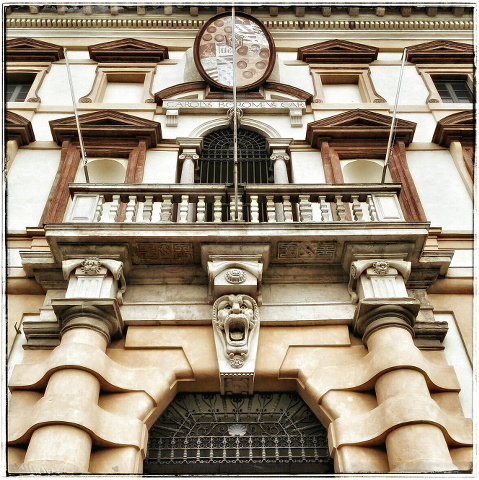
\includegraphics{smallthumb-lesson_I.jpeg}
\setfloatalignment{b}
\end{marginfigure}


\begin{abstract}
\noindent
Queste lezioni riprendono il testo introduttivo al Latino di Pearson\cite{pearson1915}, del quale seguono la numerazione; la struttura di ogni lezione è piuttosto regolare: inizia con \textsc{cenni di morfologia e di sintassi latina}, seguita da un \textsc{piccolo vocabolario} per il lessico; ci sono infine vari \textsc{esercizi} di traduzione e di composizione latina.

\bigskip
\noindent
Lezione II - Seconda Declinazione, temi in -o-, nomi maschili in -us, aggettivi maschili, vocabolario, esercizi.
\end{abstract}

%\printclassoptions

% āēīōū
% ăĕĭŏŭ

\newthought{50. Seconda Declinazione.} \textbf{dominus, -ī}, m., \textit{signore, padrone}. Radice \textbf{domino-}, tema \textbf{domin-}
\begin{fullwidth}
\begin{table}[!htbp]
  \centering
  \begin{tabular}{l l l l}
    %\toprule
	\multicolumn{3}{c}{\textsc{Singolare}} & \textsc{Uscite} \\

    \nom & domin\textbf{us}, \textit{il padrone} (soggetto)    & \hspace{20mm} & \textbf{-us} \\
    \gen & domin\textbf{ī}, \textit{del padrone}   & \hspace{20mm} & \textbf{-ī} \\
    \dat & domin\textbf{ō}, \textit{al padrone} & \hspace{20mm} & \textbf{-ō} \\
    \acc & domin\textbf{um}, \textit{il padrone} (compl.oggetto)    & \hspace{20mm} & \textbf{-um} \\
    \voc & domin\textbf{e}, \textit{o padrone}   & \hspace{20mm} & \textbf{-e} \\
    \abl & domin\textbf{ō}, \textit{per mezzo del padrone} & \hspace{20mm} & \textbf{-ō} \\
	
	\multicolumn{4}{c}{\textemdash} \\
	\multicolumn{3}{c}{\textsc{Plurale}} & \textsc{Uscite} \\

	\nom & domin\textbf{ī}, \textit{i padroni} (soggetto)    & \hspace{20mm} & \textbf{-ī} \\
    \gen & domin\textbf{ōrum}, \textit{dei padroni}   & \hspace{20mm} & \textbf{-ōrum} \\
    \dat & domin\textbf{īs}, \textit{ai padroni} & \hspace{20mm} & \textbf{-īs} \\
    \acc & domin\textbf{ōs}, \textit{i padroni} (compl.oggetto)    & \hspace{20mm} & \textbf{-ōs} \\
    \voc & domin\textbf{ī}, \textit{o padroni}   & \hspace{20mm} & \textbf{-ī} \\
    \abl & domin\textbf{īs}, \textit{per mezzo dei padroni} & \hspace{20mm} & \textbf{-īs} \\

    %\bottomrule
  \end{tabular}
  %\caption[bottom]{Prima Declinazione. \textbf{stella, -ae}, f.}
  \label{tab:normaltab}
  %\zsavepos{pos:normaltab}
\end{table}
\end{fullwidth}

\newthought{51.} Gli aggettivi maschili che escono in \textbf{-us} sono declinati come i nomi della Seconda Declinazione che escono in \textbf{-us}.

\newpage

\begin{center}
\textbf{dominus bonus}, m., \textit{il padrone buono} \\
radice \textbf{domino- bono-} \quad tema \textbf{domin- bon-}
\end{center}

\begin{fullwidth}
\begin{table}[!htbp]
  \centering
  \begin{tabular}{l l}
    %\toprule
	& \multicolumn{1}{c}{\textsc{Singolare}}\\

    \nom & domin\textbf{us} bon\textbf{us}, \textit{il padrone buono} (soggetto) \\
    \gen & domin\textbf{ī} bon\textbf{ī}, \textit{del padrone buono} \\
    \dat & domin\textbf{ō} bon\textbf{ō}, \textit{al padrone buono}  \\
    \acc & domin\textbf{um} bon\textbf{um}, \textit{il padrone buono} (compl.oggetto) \\
    \voc & domin\textbf{e} bon\textbf{e}, \textit{o padrone buono} \\
    \abl & domin\textbf{ō} bon\textbf{ō}, \textit{per mezzo del padrone buono} \\
	
	\multicolumn{2}{c}{\textemdash} \\
	& \multicolumn{1}{c}{\textsc{Plurale}}\\

	\nom & domin\textbf{ī} bon\textbf{ī}, \textit{i padroni buoni} (soggetto)  \\
    \gen & domin\textbf{ōrum} bon\textbf{ōrum}, \textit{dei padroni buoni}   \\
    \dat & domin\textbf{īs} bon\textbf{īs}, \textit{ai padroni buoni} \\
    \acc & domin\textbf{ōs} bon\textbf{ōs}, \textit{i padroni buoni} (compl.oggetto)  \\
    \voc & domin\textbf{ī} bon\textbf{ī}, \textit{o padroni buoni}  \\
    \abl & domin\textbf{īs} bon\textbf{īs}, \textit{per mezzo dei padroni buoni} \\

    %\bottomrule
  \end{tabular}
  %\caption[bottom]{Prima Declinazione. \textbf{stella, -ae}, f.}
  \label{tab:normaltab}
  %\zsavepos{pos:normaltab}
\end{table}
\end{fullwidth}


\newthought{52. Domande, osservazioni ed esercizi}
\begin{itemize}
\item[\textsc{1.}] Quali uscite sono uguali tra di loro? Quali sono uguali a quelle della Prima Declinazione?  
\item[\textsc{2.}] Osserva come il tema sia ottenuto eliminando l'uscita in \textbf{-ī} del genitivo singolare. 
\item[\textsc{3.}] Coniuga l'indicativo presente per i verbi del vocabilario qui sotto (53.).  
\end{itemize}


\newthought{53. Vocabolario} 

\begin{multicols}{2}
    \noindent \hangindent=1em \textbf{amicus, -ae}, f., \textit{amico}.  \\
    \noindent \hangindent=1em \textbf{cibus, -ī}, f., \textit{cibo}.  \\
	\noindent \hangindent=1em \textbf{dominus, -ī}, f., \textit{signore, padrone}.  \\
	\noindent \hangindent=1em \textbf{equus, -ī}, f., \textit{cavallo}.  \\
	\noindent \hangindent=1em \textbf{hortus, -ī}, f., \textit{giardino}.  \\
	\noindent \hangindent=1em \textbf{servus, -ī}, f., \textit{schiavo}.  \\
	
	\noindent \hangindent=1em \textbf{sed}, cong., \textit{ma}.  \\
	
	\noindent \hangindent=1em \textbf{magnus, -ī}, agg.m., \textit{grande, alto}.  \\
	\noindent \hangindent=1em \textbf{bonus, -ī}, agg.m., \textit{buono}.  \\
	\noindent \hangindent=1em \textbf{malus, -ī}, agg.m., \textit{malvagio}.  \\
	\noindent \hangindent=1em \textbf{parvus, -ī}, agg.m., \textit{piccolo}.  \\
	\noindent \hangindent=1em \textbf{superbus, -ī}, agg.m., \textit{superbo, orgoglioso}.  \\
	\noindent \hangindent=1em \textbf{fidus, -ī}, agg.m., \textit{fedele}.  \\
	
	\noindent \hangindent=1em \textbf{delectō}, v., \textit{io piaccio, diletto}.  \\
	\noindent \hangindent=1em \textbf{servō}, v., \textit{io tengo, conservo, metto da parte}.  \\
	
\end{multicols}
% āēīōū
% ăĕĭŏŭ

\newthought{54. Esercizi di Ripasso}
\\
\textsc{I.} \quad
\textsc{1.}~Reginae nautas laudas. \quad
\textsc{2.}~Amatisne Romam?. \quad
\textsc{3.}~Ubi nautae pugnant? \quad
\textsc{4.}~Nautae in via pugnant. \quad
\textsc{5.}~Filiam reginae non amant. \quad
\textsc{6.}~Agricolas non semper laudant.
\\
\textsc{II.} \quad
\textsc{1.}~C'è penuria di soldi nel tuo paese di nascita? \quad
\textsc{2.}~La figlia della regina accusa la donna. \quad
\textsc{3.}~Dove sono i soldi del marinaio? \quad


\newthought{55. Esercizi}
\\
\textsc{I.} \quad
\textsc{1.}~Domino; amicorum; equi. \quad
\textsc{2.}~Amicis; domini superbi; equis magnis. \quad
\textsc{3.}~Servus est amicus agricolae. \quad
\textsc{4.}~Equi sunt boni sed non magni. \quad
\textsc{5.}~Regina fidum servum laudat. \quad
\textsc{6.}~Superbum dominum non amant. \quad
\textsc{7.}~Reginae filia malum servum culpat. \quad
\textsc{8.}~Superbae in Gallia sunt puellae. \quad
\textsc{9.}~Culpasne, amice, dominum servorum? \quad
\textsc{10.}~Agricolae parvos equos non laudant. \quad
\textsc{11.}~Cibus est in horto. \quad
\textsc{12.}~Cur fidi equi dominos delectant?
\\
\textsc{II.} \quad
\textsc{1.}~Ai padroni; del cavallo; per mezzo degli schiavi. \quad
\textsc{2.}~Il cibo degli schiavi non è buono. \quad
\textsc{3.}~Il padrone è nel giardino. \quad
\textsc{4.}~Incolpa il (suo) cavallo fedele. \quad
\textsc{5.}~Il giardino è grande, ma non è buono. \quad
\textsc{6.}~O schiavo, dov'è l'amico del marinaio? \quad



\begin{figure}[!b]
  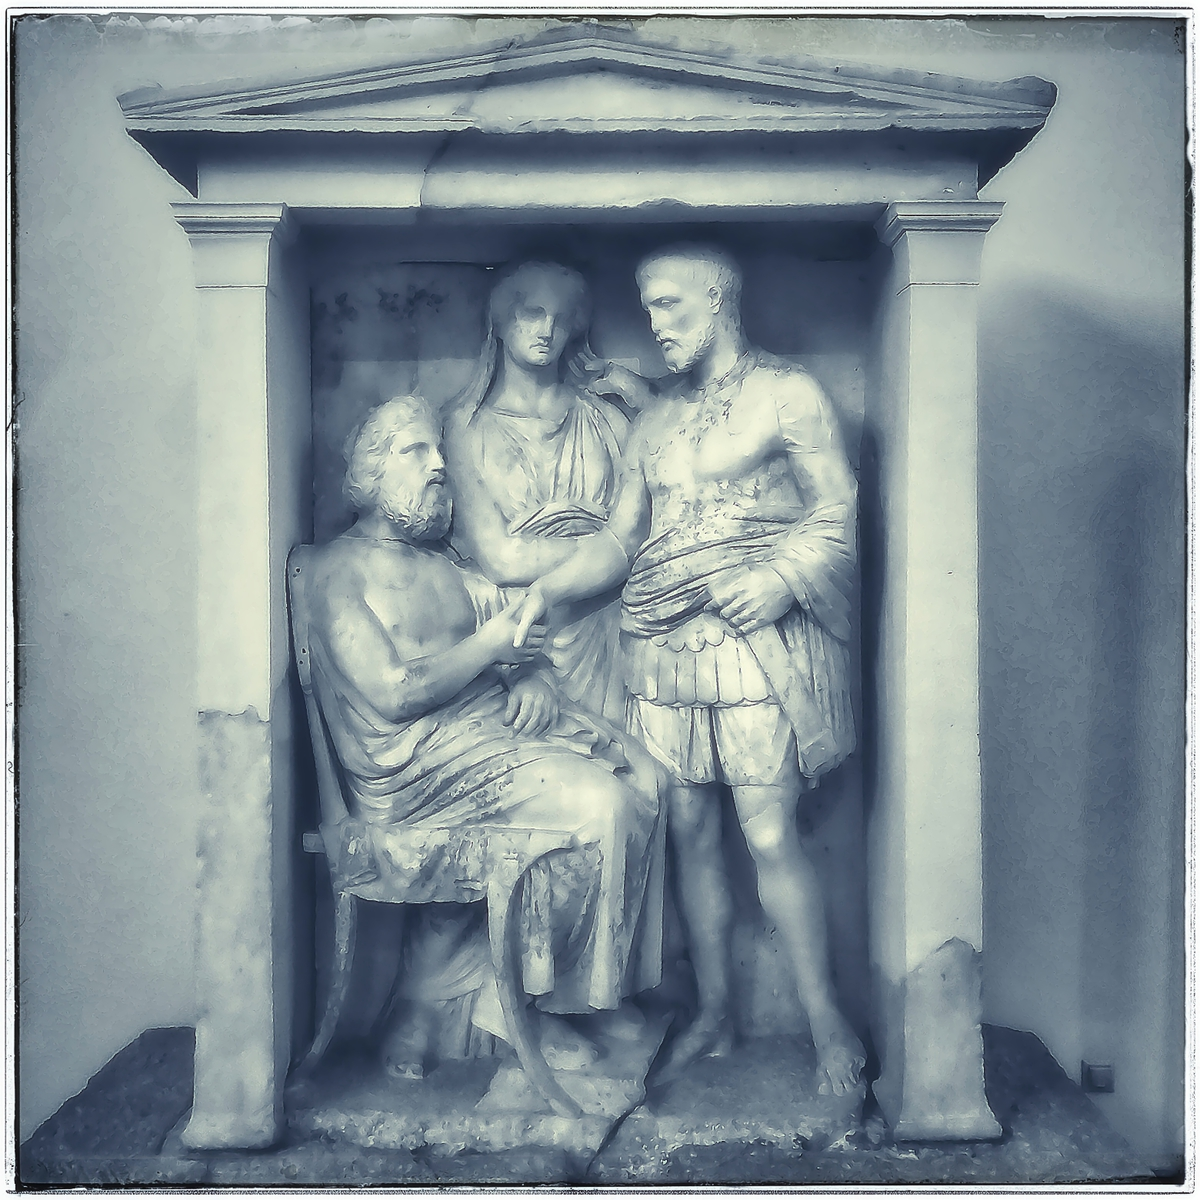
\includegraphics[width=0.8\linewidth]{thumb-lesson_V.jpeg}
  %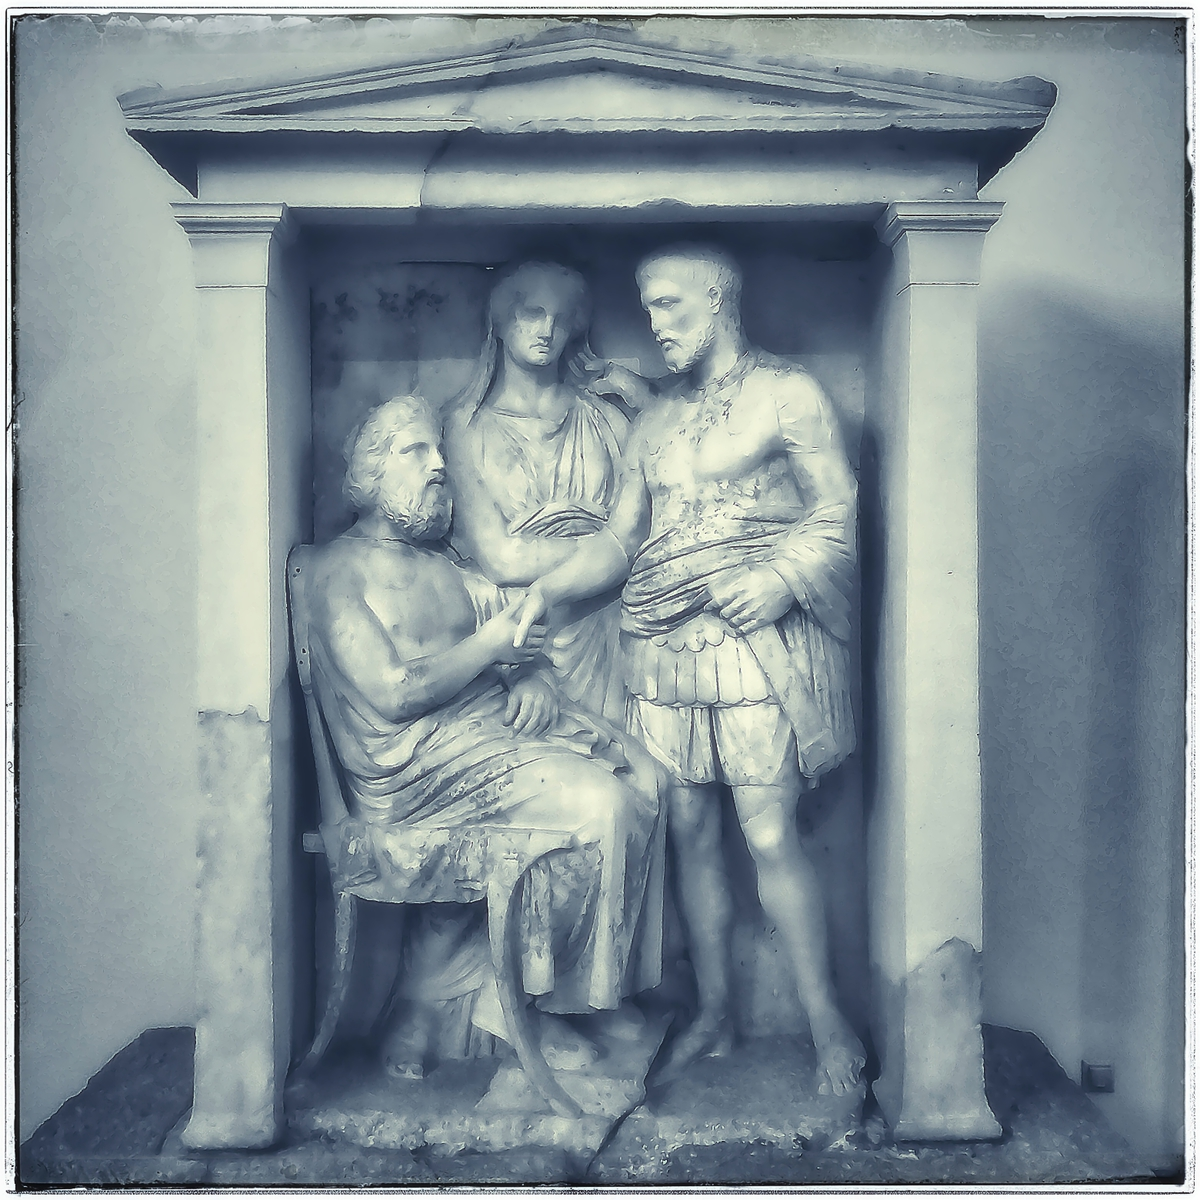
\includegraphics{thumb-lesson_V.jpeg}
  \caption{Pavia: Almo Collegio Borromeo}
  \label{fig:textfig}
  %\zsavepos{pos:textfig}
  %\setfloatalignment{b}
\end{figure}

 

\nobibliography{latinBiblio}
\bibliographystyle{alpha}


\end{document}
